%%%%%%%%%%%%%%%%%%%%%%%%%%%%%%
\chapter{Réalisation}
%%%%%%%%%%%%%%%%%%%%%%%%%%%%%%

Nous allons intégrer des digrammes d'organisation des pages Web le long de notre explication afin d'avoir un support visuel. La légende est représentée par la Figure \ref{DiagLegende}.

\begin{figure}[!ht]
	\begin{center}
		\fbox{
   		 \begin{minipage}[c]{0.4\textwidth}
  			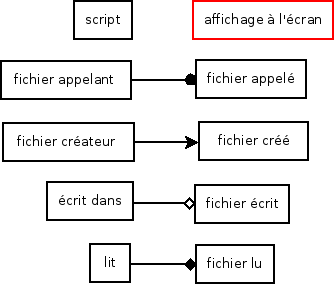
\includegraphics[width=0.90\textwidth]{../WRET/Diagramme/legende.png}  
		 \end{minipage}}
		\caption{Légende de nos diagrammes d'organisation}
  		\label{DiagLegende}
  	\end{center}	
\end{figure}

%~~~~~~~~~~~~~~~~~~~~~~~~~~~~~
\section{Ergonomie de l'interface}
%~~~~~~~~~~~~~~~~~~~~~~~~~~~~~

\subsection{Mise en page}
Nous avons utilisé le CSS afin de régler la mise en page de notre interface. Nous avons intégré une bande verticale sur la gauche du site, contenant un logo de notre création. Nous avons dû adapter la zone d'affichage en fonction de cette bande, mais également faire attention à ce que l'affichage soit ajusté à la taille de l'écran de l'utilisateur. Ce dernier critère était très important, notamment pour l'affichage du menu des onglets en haut des pages, mais aussi pour celui des pages de choix d'options de lancement. 

\paragraph*{Exemple de la page du choix des options}
Cette page est composée d'un emboîtement de plusieurs sections, grâce à la balise HTML \texttt{<div>}, qui est une sorte de conteneur. Comme nous l'avons précisé précédemment, nous avons séparé les options en plusieurs catégories et sous-catégories, distinguées par une combinaison de dégradé de bleus. 

\begin{figure}[!ht]
	\begin{center}
		\fbox{
   		 %\begin{minipage}[c]{1.1\textwidth}
  			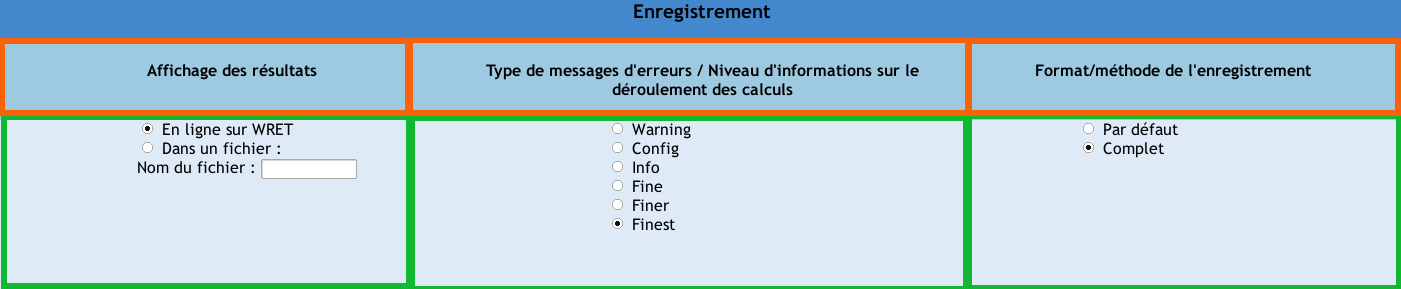
\includegraphics[width=1.0\textwidth]{../Images/Rapport/options-2.png}  
		 %\end{minipage}}
		 }
		\caption{Exemple d'organisation d'une catégorie}
  		\label{categorieCSS}
  	\end{center}	
\end{figure}

Nous avons pris l'exemple des paramètres d'enregistrement des fichiers avec trois sous-catégories, contenu dans une \textit{division}. 
\begin{itemize}
\item L'intitulé de la catégorie générale (\textit{Enregistrement}) est en bleu foncé (le même que celui de la bande verticale) et représente une sorte de \textit{sous-division}. 
\item Les titres des trois sous catégories (\textit{Affichage des résultats}, \textit{Type de messages d'erreurs} et \textit{Méthode d'enregistrement}) sont en bleu clair et représentent également une \textit{sous division}. Cette dernière est aussi divisée en trois sortes de \textit{sous-sous-division} (en orange).
\item Les contenus correspondants aux trois sous catégories sont également divisés en trois \textit{sous-sous-division} (en vert).
\end{itemize} 

Il a fallu ajuster la taille de ces sous catégories de manière relative à la taille de l'écran. Voici un exemple du code CSS correspondant:\\

\begin{DDbox}{\linewidth}
\begin{lstlisting}
div#part {
 	text-align: center;
	width:100%;
	height: 40px;
	background-color:#4388CC;
	margin-top: 30px;
	margin-bottom: 0px;
	padding: 0px;}
div#subPart {
	margin-bottom: 0px;
	margin-top: 0px;
	width:100%;
	height: 80px;
	background-color:#9ECAE1;
	padding: 0px;}
div#subPart3-2 {
	float:left;
	width:33.3%;
	height:60px;
	background-color:#9ECAE1;
	text-align: center;}
div#buttons {
	width:100%;
	height:175px;
	background-color:#DEEBF7;
	clear:both;}
div#buttons3-2 {
	float:left;
	width:33.3%;
	height:140px;
	background-color:#DEEBF7;
	text-align: justify;
	margin-right: -10%;
	margin-left: 10%;}
\end{lstlisting}
\end{DDbox}

La \texttt{div\#part} est utilisée pour le titre de la catégorie. Sa hauteur est fixe mais sa largeur s'adapte à celle de l'écran. La \texttt{div\#subPart} sert de conteneur à \texttt{div\#subPart3-1}, \texttt{div\#subPart3-2} et \texttt{div\#subPart3-3}  qui sont en vert (ici, seul le code relatif à \texttt{div\#subPart3-2} est montré pour des raisons d'économie de place car les 3 sont très semblables). De la même manière, \texttt{div\#buttons} contient \texttt{div\#buttons3-1} \texttt{div\#buttons3-2} \texttt{div\#buttons3-3} qui sont en orange. 

\subsection{Langues}
Dans un soucis de convivialité, notre interface est développée de manière à pouvoir être traduite aisément et propose trois langues possibles dans sa version actuelle (français par défaut, anglais et allemand). Pour changer la langue, l'utilisateur n'a qu'à cliquer sur le drapeau correspondant dans le menu en haut de page. Cela fera appel au script \emph{choosen\_languages.php} (Figure \ref{DiagLangues}), qui lui-même fait appel à \emph{de\_lang.php} pour l'allemand, \emph{en\_lang.php} pour l'anglais et \emph{fr\_lang.php} pour le français, en fonction du drapeau sélectionné. \\
Le fichier \emph{choosen\_languages.php} verifie  soit dans la barre d'adresse soit dans les variables de session php la langue sélectionnée par l'utilisateur.\\

\begin{DDbox}{\linewidth}
\begin{lstlisting}
session_start();
	if (isset ($_SESSION['lang']) && !isset($_GET['lang'])){
		$lang=$_SESSION['lang'];
	}
	else if (isset($_GET['lang'])){
		$lang=$_GET['lang'];
		$_SESSION['lang']=$lang;
	}
\end{lstlisting}
\end{DDbox}\\

\begin{figure}[!ht]
	\begin{center}
		\fbox{
   		 \begin{minipage}[c]{0.8\textwidth}
  			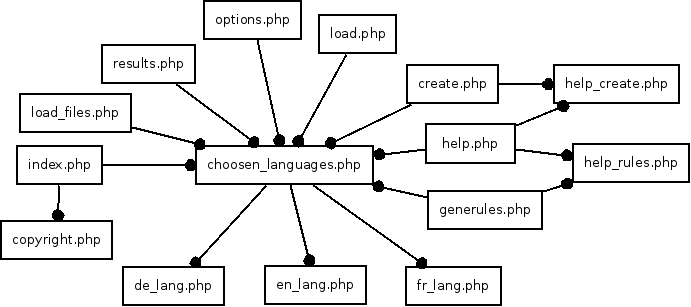
\includegraphics[width=0.90\textwidth]{../WRET/Diagramme/langues.png}  
		 \end{minipage}}
		\caption{Diagramme d'organisation pour le changement de langue}
  		\label{DiagLangues}
  	\end{center}	
\end{figure}

Pour ce faire, nous n'avons pas mis de texte dans le code des pages affichant à l'écran. Nous l'avons remplacé par des variables, qui afficheront le texte qu'elles contiennent dans la langue désirée. Par exemple, le titre de la page d'accueil "Bienvenue sur WebRegEfmTool" est appelé par \texttt{<?php echo TXT\_HOMEPAGE\_TITLE; ?>} et est contenu dans le fichier \emph{fr\_lang.php} de la manière suivante :
\texttt{define('TXT\_HOMEPAGE\_TITLE', 'Bienvenue sur WebRegEfmTool');}. De ce fait, un nouveau fichier du type \emph{XX\_lang.php} pourrait être créé afin d'intégrer une nouvelle langue. Bien sûr, il faudrait ajouter les appels à ce fichier dans toutes les pages affichant à l'écran par la suite. 

%~~~~~~~~~~~~~~~~~~~~~~~~~~~~~
\section{Création d'un nouveau réseau}
%~~~~~~~~~~~~~~~~~~~~~~~~~~~~~

\subsection{Initialisation des fichiers}
La création d'un nouveau réseau dans WRET se fait via la page \emph{create.php}.
A partir de cette page, l'utilisateur doit dans un premier temps appuyer sur le bouton \emph{Initialiser les fichiers} (Figure \ref{boutonInit}) s'il désire initialiser ses fichiers.

\begin{figure}[!ht]
    \begin{center}
        \fbox{
            \begin{minipage}[c]{0.5\textwidth}
              
\includegraphics[width=0.90\textwidth]{../Images/Rapport/creation1-1.png} 
         \end{minipage}}
        \caption{Bouton d'initialisation des fichiers}
          \label{boutonInit}
      \end{center}   
\end{figure}

Ce bouton appelle le fichier \emph{initfiles.php} qui va créer les 11 fichiers nécessaires à la mise en place d'un nouveau réseau.\\
Dans ces fichiers, nous trouvons des fichiers qui seront utilisés dans le lancement de \emph{regEfmtool} (rfile, mfile, rvfile, sfile) et également des fichiers temporaires (\emph{irrevTemp}, \emph{revTemp}, \emph{reactionTemp.txt}, \emph{reactionTemp2.txt}, \emph{matrice.txt} ou encore \emph{matrice2.txt} ainsi que la base du fichier au format \emph{DAT}).\\
Tous ces fichiers sont donc créés et donnent les droits d'édition, de lecture et d'exécution à tous les utilisateurs pour chacun d'entre eux, afin de pouvoir être modifiés sur le serveur.

\subsection{Réactions et réversibilité}
Sous la touche \emph{Initialiser les fichiers} de la page \emph{create.php}, une fenêtre de texte permet de rentrer les réactions du réseau métabolique une à une ainsi que la réversibilité de la réaction (Figure \ref{boutonAjout}).

\begin{figure}[!ht]
    \begin{center}
        \fbox{
            \begin{minipage}[c]{0.7\textwidth}
              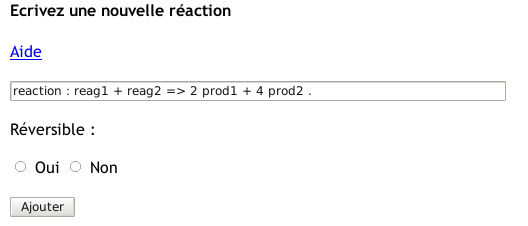
\includegraphics[width=0.90\textwidth]{../Images/Rapport/creation1-2.png} 
         \end{minipage}}
        \caption{Bouton d'ajout d'une réaction}
          \label{boutonAjout}
      \end{center}   
\end{figure}

Si l'utilisateur oublie de cocher la réversibilité de la réaction et clique sur \emph{Ajouter}, un message d'erreur s'affichera et empêchera le passage à l'étape suivante. Les réactions doivent être enregistrées par l'utilisateur en respectant la syntaxe des fichier au format \emph{DAT}. Ces informations vont alors être envoyées au fichier \emph{createFiles.php}, via le bouton \emph{Ajouter}.\\
Ce fichier redirige vers différentes pages, dans l'ordre : \emph{reac.php}, \emph{parser\_enzyme.php},
\\ \emph{parser\_reversibility.php}, \emph{parser\_metabolite.php}, \emph{parser\_stoechiometry.php}.
La première page \emph{reac.php} va permettre d'écrire dans un fichier temporaire (\emph{reactionTemp.txt}) les réactions, et également, de sauvegarder la réversibilité de la réaction (0 pour non réversible, et 1 pour réversible).\\
L'ordre est ainsi conservé entre les réactions et leur réversibilité.

\subsection{Nom de réactions : enzymes}
Une fois les données de réactions et de réversibilité enregistrées, la page \emph{parser\_enzymes.php} est appelée. Elle va parser le fichier temporaire des réactions (\emph{reactionTemp.txt}) et va extraire le premier élément de la réaction situé avant le ": ", qui se trouve être le nom de la réaction (nom de l'enzyme généralement).\\
Ces noms sont enregistrés dans un fichier (\emph{reactions.rfile}) en respectant les espaces et la syntaxe nécessaires à son utilisation au sein de \emph{regEfmtool}.

\subsection{Métabolites}
Après enregistrement des enzymes, le fichier \emph{parser\_metabolites.php} est appelé. Ce script va parser le fichier temporaire contenant les réactions (\emph{reactionTemp.txt}) et va enregistrer chacun des métabolites dans un fichier (\emph{metabolites.mfile}). Au cours de ce parsage, seuls les éléments situés après le nom de l'enzyme seront pris en compte. Les noms présents plusieurs fois dans le fichier de réactions sont enregistrés une seule fois dans le fichier \emph{metabolites.mfile}.

\subsection{Stœchiométrie}
Enfin après génération des fichiers: \emph{rvfile}, \emph{mfile}, \emph{sfile}, \emph{rfile}, le script \emph{parser\_stoechiometry} est appelé. Il va lancer le script \emph{parser\_stoechiometry.py}. Ce dernier permet de générer la matrice de stœchiométrie nécessaire à \emph{regEfmtool}. Pour ce faire, il prend les fichiers \emph{reactionTemp.txt} et \emph{metabolites.mfile} en entrée. Il génère la matrice ligne par ligne (une ligne correspondant à une réaction). \\
Pour chaque ligne du fichier \emph{reactionTemp.txt}, une liste est créée et, pour chaque métabolite de cette réaction, sa stœchiométrie est enregistrée en respectant son ordre dans le fichier contenant les réactifs. Ce script fourni alors en sortie le fichier \emph{stoechiometry.sfile}.

\subsection{Modification du réseau}
Une fois les fichiers générés, l'utilisateur est redirigé vers la page \emph{create.php}.
Sous la touche \emph{Ajouter} se trouve une zone de texte (Figure \ref{boutonAjout}) où l'utilisateur peut modifier un réseau déjà rentré.

\begin{figure}[!ht]
    \begin{center}
        \fbox{
            \begin{minipage}[c]{0.7\textwidth}
              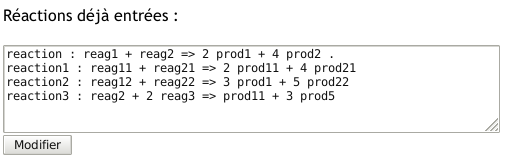
\includegraphics[width=0.90\textwidth]{../Images/Rapport/creation1-3.png} 
         \end{minipage}}
        \caption{Bouton de modification}
          \label{boutonModif}
      \end{center}   
\end{figure}

En effet, cette zone appelle le fichier \emph{reactionTemp.txt} et permet la modification de son contenu (pour corriger une erreur de frappe notamment). Cette zone de texte va appeler la page \emph{modifier.php} lors de l'utilisation du bouton \emph{Modifier}.\\
 Cette page efface le précédent fichier \emph{reactionTemp.txt} et insère le nouveau contenu que l'utilisateur a modifié. \\
 Les fichiers \emph{metabolites.mfile}, \emph{stoechiometry.sfile}, \emph{reactions.rfile}, \emph{reversibility.rvfile}, sont également générés à nouveau, à chaque modification du fichier \emph{reactionTemp.txt}.
 
\subsection{Création du fichier \emph{DAT}}

En dessous de la zone de texte modifiable, une touche nommée \emph{Choisir les métabolites internes et externes} (Figure \ref{boutonMET_int_EXT}) permet à l'utilisateur de définir dans son réseau les métabolites internes et externes. Ce bouton va effectuer un parsage du fichier \emph{metabolites.mfile} et afficher dans une colonne à gauche tous les métabolites. Une colonne à droite vide peut être remplie ou vidée via les boutons \emph{Ajouter}, \emph{Supprimer} situés entre les colonnes.
Ces touches d'ajout et de suppression font appelle à des fonctions \emph{JavaScript}, directement intégrées à la page \emph{create.php}.\\

\begin{figure}[!ht]
    \begin{center}
        \fbox{
            \begin{minipage}[c]{0.5\textwidth}
              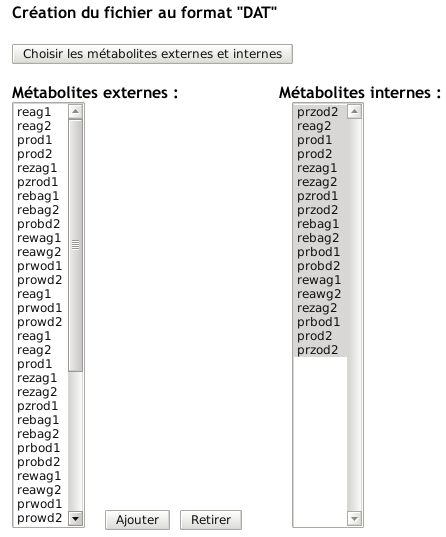
\includegraphics[width=0.9\textwidth]{../Images/Rapport/creation3.png} 
         \end{minipage}}
        \caption{Zone de sélection des métabolites internes et externes}
          \label{boutonMET_int_EXT}
      \end{center}   
\end{figure}

Sous la zone de sélection des métabolites internes et externes, un bouton \emph{DAT} permet de générer un fichier au format \emph{DAT} du réseau métabolique précédemment créé. \\

\begin{figure}[!ht]
    \begin{center}
        \fbox{
            \begin{minipage}[c]{0.3\textwidth}
              
\includegraphics[width=0.90\textwidth]{../Images/Rapport/creation2-1.png} 
         \end{minipage}}
        \caption{Bouton de création du fichier au format \emph{DAT}}
          \label{boutonDAT}
      \end{center}   
\end{figure}

Ce bouton (Figure \ref{boutonDAT}) appelle la page \emph{finish\_files.php} qui va  récupérer les choix de l'utilisateur en ce qui concerne les métabolites internes et externes, et concaténer trois fichiers :
\begin{itemize}
\item \emph{irrevTemp.txt}
\item \emph{revTemp.txt}
\item \emph{reactiontemp2.txt}
\end{itemize}

Le premier fichier contient l'ensemble des enzymes catalysant les réactions irréversibles. Le second contient l'ensemble des enzymes catalysant les réactions réversibles, et enfin le dernier fichier contient l'ensemble des réactions du réseau. \\
Chacun de ces fichiers contient les balises \emph{-ENZIRREV}, \emph{-ENZREV}, \emph{-CAT}, selon son contenu et respecte la syntaxe propre au format \emph{DAT}.
Les noms des métabolites sont insérés dans le fichier au format \emph{DAT} après une balise \emph{-METINT} ou \emph{-METEXT}, selon leur rôle dans le réseau défini par l'utilisateur.

Il en résulte en sortie du script \emph{finish\_files.php} un fichier au format \emph{DAT}, de la forme:
\\
\begin{DDbox}{\linewidth}
\begin{lstlisting}
-ENZREV
R9 R12 R13 R14 R15   T1 T2 T5 T7 T12

-ENZIRREV
R6i R7i R8i R10i R11i T6

-METINT
OAA ACoA Cit Akg SucCoA Succ Fum Mal Isocit  Pi  Glu Asp Pyr

-METEXT
Pyr_ext Glu_ext NAD NADH2 FAD FADH2  CoA ADP ATP  H2O CO2 Mal_ext Cit_ext AKG_ext Pi_ext Asp_ext

-CAT

R6i : Pyr + CO2 + ATP = OAA + Pi + ADP .
R7i : Pyr + NAD + CoA = ACoA + NADH2 + CO2 .
R8i : OAA + ACoA + H2O = Cit + CoA .
R9 : Cit = Isocit .
R10i : Isocit + NAD = Akg + NADH2 + CO2 .
R11i : Akg + NAD + CoA = SucCoA + NADH2 + CO2 .
R12 : SucCoA + Pi + ADP = Succ + CoA + ATP .
R13 : Succ + FAD = Fum + FADH2 .
R14 : Fum + H2O = Mal .
R15 : Mal + NAD = OAA + NADH2 .
T1 : Cit + Mal_ext = Mal + Cit_ext .
T2 : AKG_ext + Mal = Mal_ext + Akg .
T5 : Pi_ext = Pi .
T6 : Pyr_ext = Pyr .
T7 : Mal + Pi_ext = Pi + Mal_ext .
T12 : Asp + Glu_ext = Asp_ext + Glu .

\end{lstlisting}
\end{DDbox}

%~~~~~~~~~~~~~~~~~~~~~~~~~~~~~
\section{Règles des gènes}
%~~~~~~~~~~~~~~~~~~~~~~~~~~~~~

\begin{figure}[!ht]
	\begin{center}
		\fbox{
   		 \begin{minipage}[c]{0.7\textwidth}
  			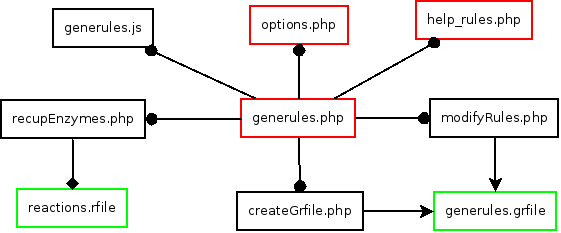
\includegraphics[width=0.90\textwidth]{../WRET/Diagramme/generules.png}  
		 \end{minipage}}
		\caption{Diagramme d'organisation pour le changement de langue}
  		\label{DiagRegles}
  	\end{center}	
\end{figure}

La page permettant la saisie des règles générales est obtenue à l'aide du fichier \emph{generules.php} (Figure \ref{DiagRegles}).\\
L'affichage à l'ouverture de la page n'est composé que d'une zone de texte et d'un bouton \emph{Ok} (Figure \ref{boutonOK}) qui est de type \textit{submit}. 

\begin{figure}[!ht]
	\begin{center}
		\fbox{
   		 \begin{minipage}[c]{0.3\textwidth}
  			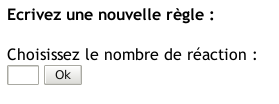
\includegraphics[width=0.90\textwidth]{../Images/Rapport/generules-1.png}  
		 \end{minipage}}
		\caption{Bouton du choix du nombre de réactions pour une règle}
  		\label{boutonOK}
  	\end{center}	
\end{figure}

Au clic, ce bouton fait appel à la fonction \emph{add\_reaction()} qui créée  deux menus déroulants (pour la première et la dernière, Figure \ref{menusDeroulants1}) ou trois menus déroulants (pour les autres, Figure \ref{menusDeroulants2}) par réaction jusqu'à atteindre le nombre de réactions entrées par l'utilisateur. 

\begin{figure}[!ht]
	\begin{center}
		\fbox{
   		 \begin{minipage}[c]{0.7\textwidth}
  			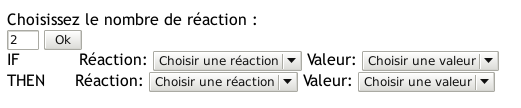
\includegraphics[width=0.90\textwidth]{../Images/Rapport/generules-2.png}  
		 \end{minipage}}
		\caption{Menus déroulant si 2 réactions dans la règle}
  		\label{menusDeroulants1}
  	\end{center}	
\end{figure}

\begin{figure}[!ht]
	\begin{center}
		\fbox{
   		 \begin{minipage}[c]{0.8\textwidth}
  			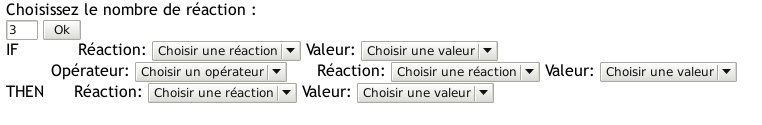
\includegraphics[width=0.90\textwidth]{../Images/Rapport/generules-3.png}  
		 \end{minipage}}
		\caption{Menus déroulant si 3 réactions dans la règle}
  		\label{menusDeroulants2}
  	\end{center}	
\end{figure}

Elle vérifie également que le nombre de réactions entrées par l'utilisateur est au moins égal à 2, sinon elle affiche un message sous la forme d'une alerte à l'utilisateur.\\
Les réactions sont récupérées à partir de \emph{reactions.rfile}.\\

L'utilisateur peut sélectionner plusieurs fois la m\^eme réaction dans sa règle, sauf pour le choix de la dernière (ligne THEN). Cette particularité est gérée par la fonction \texttt{choice(form, val)}. Celle-ci permet de remplir les menus déroulants quand une réaction a été choisie et pour la dernière seules les réactions non sélectionnées précédemment appara\^issent.

Lorsque l'utilisateur a choisi toutes ses réactions, leur opérateur et leur valeur, il clique sur le bouton \emph{Ajouter}. Celui-ci fait appel à la fonction \texttt{validateForm()} qui vérifie que tous les champs ont bien été sélectionnés. Si la fonction retourne VRAI, il fait appel au fichier \emph{createGrfile.php} qui écrit la règle dans le fichier \emph{generules.grfile}.\\
Le fichier \emph{createGrfile.php} écrit dans le fichier \emph{grfile} selon certaines règles. En effet, l'écriture de la règle dépend des valeurs associées aux réactions et des opérateurs choisis.\\

Si la valeur de la réaction qui suit le "THEN" est 0, alors il y aura le symbole "!" au début de la règle (juste après le "="), sauf si la règle ne contient que deux réactions.\\
Si les autres réactions ont pour valeur:
\begin{itemize}
\item 0, alors on écrira (!0reac)
\item 1, alors on écrira (!1reac)
\item f, alors on écrira (!freac)
\end{itemize}
En revanche, si la valeur de la réaction après "THEN" est 1, les autres réactions s'écriront:
\begin{itemize}
\item 0reac si sa valeur est 0
\item 1reac si sa valeur est 1
\item freac si sa valeur est f
\end{itemize}
De plus, si l'opérateur "AND" est sélectionné il sera écrit sous la forme \& dans le fichier, l'opérateur "OR" sera lui écrit $|$. Quand la règle est composée d'au moins trois réactions, des parenthèses sont ajoutées après chaque réaction sauf la première et la dernière. Des parenthèses entourent l'ensemble des réactions situées après le "=".\\

Pour mieux comprendre l'écriture du fichier \emph{generules.grfile}, voici un exemple:\\

Choix de l'utilisateur sur la page Web: \\
\begin{DDbox}{\linewidth}
\begin{lstlisting}
IF reaction: R1 valeur: 1
Operateur: AND reaction: R2 valeur: 0
Operateur: OR reaction: R3 valeur: 0
THEN reaction: R4 valeur: 0
\end{lstlisting}
\end{DDbox}

Règle écrite dans le fichier: \\
\begin{DDbox}{\linewidth}
\begin{lstlisting}
R4 = (!((1R1 & (!0R2)) | (!0R3))
\end{lstlisting}
\end{DDbox}

%~~~~~~~~~~~~~~~~~~~~~~~~~~~~~
\section{Choix des options de lancement}
%~~~~~~~~~~~~~~~~~~~~~~~~~~~~~

\begin{figure}[!ht]
	\begin{center}
		\fbox{
   		 \begin{minipage}[c]{0.6\textwidth}
  			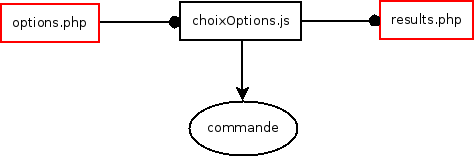
\includegraphics[width=0.90\textwidth]{../WRET/Diagramme/options.png}  
		 \end{minipage}}
		\caption{Diagramme d'organisation pour le choix des options après création}
  		\label{DiagOptions}
  	\end{center}	
\end{figure}

La page permettant la sélection des options de lancement est obtenue à l'aide du fichier \emph{options.php} (Figure \ref{DiagOptions}). Comme nous l'avons dit précédemment, nous avons séparé les options en une série de catégories et sous catégories, le tout contenu dans un formulaire afin de gérer l'interaction avec l'utilisateur. Ce dernier peut sélectionner les options qu'il désire avec une combinaison de \textit{radioboutons} et de zones de texte. Les \textit{radioboutons} d'une même sous-section ont le même attribut \textit{name} afin de ne pouvoir en sélectionner qu'un seul. \\

Prenons comme exemple la première sous catégorie (Figure \ref{affichageResults}) :

\begin{figure}[!ht]
	\begin{center}
		\fbox{
   		 \begin{minipage}[c]{0.3\textwidth}
  			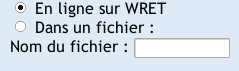
\includegraphics[width=0.90\textwidth]{../Images/Rapport/options-1.png}  
		 \end{minipage}}
		\caption{Sous catégorie d'affichage des résultats dans la catégorie d'enregistrement}
  		\label{affichageResults}
  	\end{center}	
\end{figure}

Voici le code HTML/PHP qui correspond :

\scriptsize
\begin{DDbox}{\linewidth}
\begin{lstlisting}
<input type="radio" name="choix1" value="log console" checked="checked">	<?php echo TXT_OPTIONS_SAVING_3; ?> 
<input type="radio" name="choix1" value="log file"> <?php echo TXT_OPTIONS_SAVING_4; ?> 
<?php echo TXT_OPTIONS_SAVING_5; ?> <input type="text"	 name="log_nomFichier" 	size="10" id="texte1">
\end{lstlisting}
\end{DDbox}

\normalsize

Le premier \textit{radiobouton} est pré-coché avec l'attribut \textit{checked="checked"} afin de guider l'utilisateur. Si cette option ne lui convient pas, il lui suffit de cocher le deuxième \textit{radiobouton} et de remplir la zone de texte associée. \\

Ce sont les attributs \textit{value} de ces boutons qui sont récupérés avec un script \emph{JavaScript}. Ce dernier, nommé \emph{choixOptions.js}, permet de vérifier quels \textit{radioboutons} sont cochés et récupère ce qu'il a dans l'attribut \textit{value} de ceux-ci quand c'est le cas. Il est appelé lors du clic sur le bouton \textit{Lancement} en bas de la page. De plus, c'est dans ce script qu'est générée la commande qui permettra le lancement de regEfmtool. Elle est contenue dans une variable nommée  \textit{commande}, qui se remplit grâce aux paramètres sélectionnés. \\

Exemple du code \emph{JavaScript} qui permet la récupération des \textit{values} précédentes : \\

\begin{DDbox}{\linewidth}
\begin{lstlisting}
var commande = "java -Xmx1G -jar ../regEfmtool.jar";

  // SAVE
  // Display
  if (formulaire.choix1[0].checked) { 
    valeur1 = " -" + formulaire.choix1[0].value; 
    commande = commande + valeur1;
  }
  else if (formulaire.choix1[1].checked) { 
    var nom1 = document.getElementById('texte1').value;
    valeur1 = " -" + formulaire.choix1[1].value + " " + nom1; 
    commande = commande + valeur1;
  }
\end{lstlisting}
\end{DDbox}

La variable \textit{commande} est une chaîne de caractères qui contient le début de la commande Java. Les paramètres sont ensuite ajoutés au fur et à mesure de la vérification de la sélection des boutons. \\

Cette commande est sauvegardée dans un \textit{cookie} qui sera récupéré à la page d'affichage des résultats pour le lancement de regEfmtool. 

%~~~~~~~~~~~~~~~~~~~~~~~~~~~~~
\section{Chargement d'un réseau pré-existant}
%~~~~~~~~~~~~~~~~~~~~~~~~~~~~~

\begin{figure}[!ht]
	\begin{center}
		\fbox{
   		 \begin{minipage}[c]{0.7\textwidth}
  			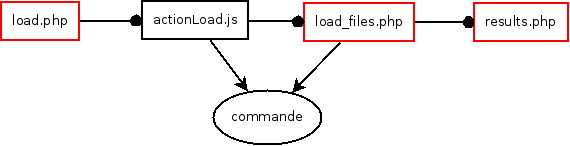
\includegraphics[width=0.90\textwidth]{../WRET/Diagramme/load.png}  
		 \end{minipage}}
		\caption{Diagramme d'organisation pour le chargement des fichiers}
  		\label{DiagLoad}
  	\end{center}	
\end{figure}

Ce sont les pages \emph{load.php} et \emph{load\_files.php} qui permettent le chargement des fichiers contenant un réseau pré-existant (Figure \ref{DiagLoad}) depuis le disque dur de l'utilisateur.\\

Tout d'abord, la page \emph{load.php} permet à ce dernier de choisir les paramètres de la commande de lancement de \textit{regEfmtool}, de le même façon que pour la page \emph{options.php}. Cependant, la deuxième grande catégorie diffère car le choix des fichiers à charger se fera lors d'une étape ultérieure. Ici, l'utilisateur coche les options qu'il désire et clique sur le bouton \textit{Étape suivante}. Ce bouton fait appel au script \emph{JavaScript} \emph{actionLoad.js}, qui fonctionne sur le même principe que \emph{choixOptions.js}. \\

Ensuite, l'utilisateur est dirigé vers la page \emph{load\_files.php}, qui permet à l'utilisateur d'aller "chercher" les fichiers aux formats \textit{sfile}, \textit{mfile}, \textit{rvfile}, \textit{grfile} et \textit{rfile}. Nous copions et renommons ces fichiers dans le dossier courant afin de pouvoir les utiliser dans \textit{regEfmtool}. Ce processus est faisable grâce à un  script PHP, dont voici un exemple pour le fichier au format \textit{sfile} :\\

\begin{DDbox}{\linewidth}
\begin{lstlisting}
 move_uploaded_file($_FILES["sfile"]["tmp_name"],$_FILES["sfile"]["name"]);
 shell_exec('mv ' . $_FILES["sfile"]["name"] . ' sfile');
\end{lstlisting}
\end{DDbox}

Ce script est contenu dans l'attribut \textit{value} du bouton de chargement du fichier en question. La ligne de commande est donc complétée et le lancement du logiciel peut commencer. 

%~~~~~~~~~~~~~~~~~~~~~~~~~~~~~
\section{Affichage des résultats}
%~~~~~~~~~~~~~~~~~~~~~~~~~~~~~

\begin{figure}[!ht]
	\begin{center}
		\fbox{
   		 \begin{minipage}[c]{0.6\textwidth}
  			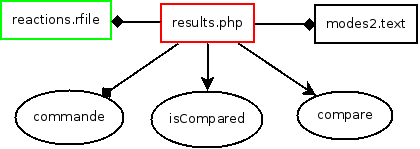
\includegraphics[width=0.90\textwidth]{../WRET/Diagramme/results.png}  
		 \end{minipage}}
		\caption{Diagramme d'organisation pour l'affichage des résultats}
  		\label{DiagResults}
  	\end{center}	
\end{figure}

Le fichier \emph{results.php} permet l'affichage des résultats de la commande générée précédemment. Celle-ci est exécutée grâce à la fonction \texttt{shell\_exec()}. Les fichiers de résultat et de log sont analysés pour permettre leur affichage (Figure \ref{DiagResults}).\\

\begin{figure}[!ht]
	\begin{center}
		\fbox{
   		 \begin{minipage}[c]{0.8\textwidth}
  			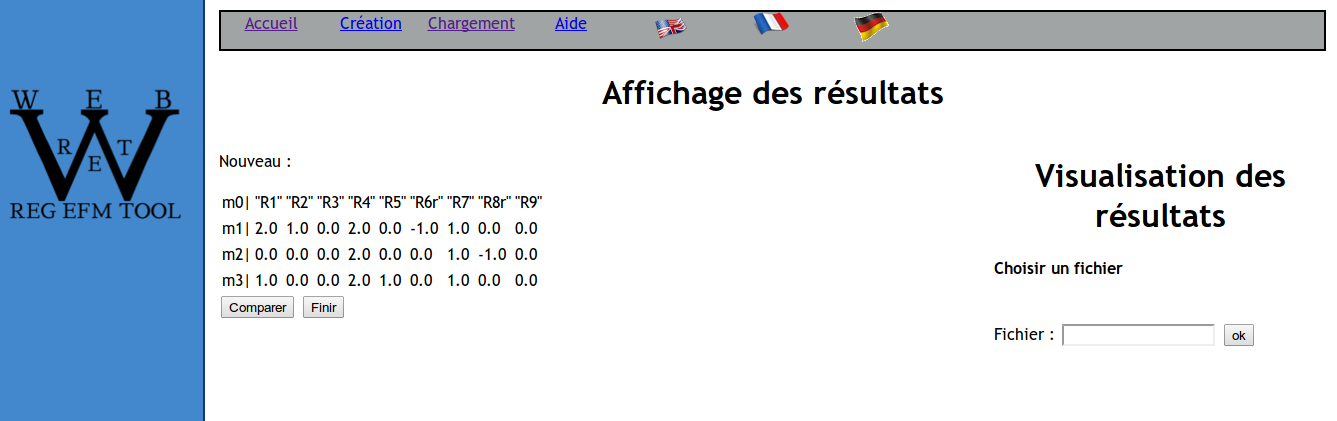
\includegraphics[width=0.9\textwidth]{../Images/Rapport/results.png}  
		 \end{minipage}}
		\caption{Page d'affichage des résultats}
  		\label{Results}
  	\end{center}	
\end{figure}

L'affichage (Figure \ref{Results}) se fait en plusieurs étapes : tout d'abord, nous vérifions grâce à la variable de session PHP \texttt{isCompared} si l'utilisateur veut afficher un ou plusieurs résultats.\\

Prenons le cas d'un utilisateur qui calcule une première fois les modes élémentaires d'un réseau : la variable \texttt{isCompared} indique à l'interface qu'il n'y a qu'un résultat à afficher, la \texttt{<div id='new'>} est créée. Nous affichons tout d'abord une image \emph{waiting.gif} grâce à la fonction \texttt{waiting()}, qui se charge aussi d'exécuter la commande précédemment conservée dans les cookies HTML .\\

\begin{DDbox}{\linewidth}
\begin{lstlisting}
function waiting(){
	echo ('<img src="Images/waiting.gif" alt="please Wait...">');
	$com = $_COOKIE['commande'];
	if ($_SESSION['isCompared']==1) {
		$com =  $com . ' > log.txt';
		shell_exec($com);
	}
	else {
		$com = $com . ' > log1.txt';
		shell_exec($com);
	}
}
\end{lstlisting}
\end{DDbox}\\

Cette fonction vérifie donc si l'utilisateur voulait comparer son résultat et sauvegarde le log dans le fichier \emph{log1.txt} ou \emph{log.txt} suivant le cas.\\

\begin{DDbox}{\linewidth}
\begin{lstlisting}
<div id="new" name="new" title="new results">
	<?php
		if (count($modes)<2)
			echo '<script>document.getElementById("new").innerHTML = "";</script>';
			waiting();
		}
		$res2=parse_res();
		echo '<script>document.getElementById("new").innerHTML = "";</script>';
		echo '<p>' . TXT_DISPLAY_RESULTS_NEW . '</p>';
		show_results($res2);
		$_SESSION['compare']=$res2;
	?>		
\end{lstlisting}
\end{DDbox}

Ensuite, nous effectuons un parsage du résultat avec la fonction \texttt{parse\_res()} qui ouvre le fichier de résultats généré et le sauvegarde dans un tableau pour faciliter son affichage. \\
Finalement, la fonction \texttt{show\_res(resultat)} permet d'afficher le résultat en ajoutant au tableau les noms des réactions, ainsi qu'une colonne indiquant le mode. \textbf{\textcolor{red}{mode élémentaire ??}} \\
Dans le cas où l'utilisateur souhaite comparer deux résultats, une \texttt{<div id'original'>} HTML est créée (Figure \ref{comparaison}). Celle-ci contient le premier résultat calculé et nous continuons avec le nouveau résultat à afficher.\\

\begin{DDbox}{\linewidth}
\begin{lstlisting}
if ($_SESSION["isCompared"]==1){
	$res=$_SESSION["compare"];
	echo "<div id='original' name='original' title='original results' >";
	echo '<p>' . TXT_DISPLAY_RESULTS_ORIGINAL . '</p>';
	show_results($res);
	echo "</div>";
}
\end{lstlisting}
\end{DDbox}

\begin{figure}[!ht]
    \begin{center}
        \fbox{
            \begin{minipage}[c]{0.9\textwidth}
              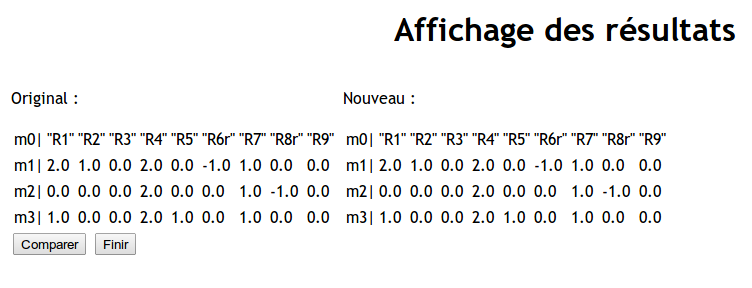
\includegraphics[width=0.9\textwidth]{../Images/Rapport/results_compare.png} 
         \end{minipage}}
        		\caption{Exemple de comparaison de deux résultats}
          \label{comparaison}
      \end{center}   
\end{figure}

Une fois toutes ces étapes finies, le résultat est sauvegardé dans la variable \texttt{compare} pour le cas où l'utilisateur voudrait comparer son résultat avec un autre (avec par exemple des choix différents d'options, de nouvelles règles).\\

L'utilisateur a donc le choix de terminer ses calculs ou de comparer le résultat obtenu. Pour cela, deux boutons \textit{Comparer} et \textit{Finir} lui permettent de retourner à l'écran d'accueil. Cependant, \textit{Comparer} fait appel à la fonction \texttt{compare()}  qui conserve en mémoire le fait que l'utilisateur veut comparer son résultat. Ceci est possible grâce à une variable de session PHP \texttt{isCompared}. Le bouton \textit{Finir} quant à lui réinitialise cette m\^eme variable avant d'effectuer la redirection.\\

Sur cette même page, l'utilisateur a aussi la possibilité d'afficher les résultats de la commande qu'il vient de lancer. Pour cela, le fichier \emph{parse\_results.php} récupère le fichier \emph{log.txt} dans lequel les résultats générés par \textit{regEfmtool} ont été redirigés. \\

Cette page offre deux options:
\begin{itemize}
\item visualiser l'ensemble des résultats ,
\item choisir une catégorie de résultats à visualiser.
\end{itemize}

Cette page parcourt le fichier log et sélectionne les mots-clés à l'aide de la fonction \texttt{item()}, qui récupère toute les phrases suivies de "\texttt{:}".

\begin{DDbox}{\linewidth}
\begin{lstlisting}
function item(){
					
	$fichier = 'log.txt';
	global $item;
	define ('FICHIER', $fichier);
	$numligne = 0;

	$fichier = fopen( FICHIER, 'r')or die('Ouverture en lecture de "' . FICHIER . '" impossible !');
					
	while (!feof($fichier)){
		$numligne++;
		$lignes = fgets($fichier, 1024);
		$posi = strpos($lignes, '|'); 
		$ligne = trim(substr($lignes,$posi+1,strlen($lignes))); 
		$pos = strpos($ligne, ':' );
		if ( $pos == true && $numligne >= 32){
			$line = trim(substr($ligne,0, $pos)); 
			$item[] = $line;
		}
	}
					
	$count = count($item);
					
	for ($numero = 0; $numero < $count; $numero++){
		echo '<OPTION VALUE="' . $item[$numero] . '"> ' . $item[$numero] . ' </OPTION>'; 
	}
	return $item;
}
\end{lstlisting}
\end{DDbox}

Les mots-clés sont stockés dans un menu déroulant, qui est obtenu par affichage de chaque valeur du tableau dans la balises HTML \texttt{'<OPTION VALUE="' . $item[$numero] . '"> ' . $item[$numero] . ' </OPTION>'}. Ainsi l'utilisateur n'a plus qu'à sélectionner la catégorie qu'il souhaite visualiser à partir du mot-clé. \\

Ainsi la visualisation peut se faire sur l'ensemble du fichier \emph{log.txt} (Figure \ref{affichageResultats}) et une redirection sur la page  \emph{all\_results.php} sera effectuée. La visualisation peut également se faire sur une seule catégorie et la redirection sera alors sur \emph{display\_results.php}. De plus, la page d'affichage des résultats offre la possibilité à l'utilisateur de revenir en arrière à l'aide de deux boutons, dont un présent au-dessus de l'affichage des résultats et l'autre, en-dessous.\\

\begin{figure}[!ht]
	\begin{center}
		\fbox{
   		 \begin{minipage}[c]{0.8\textwidth}
  			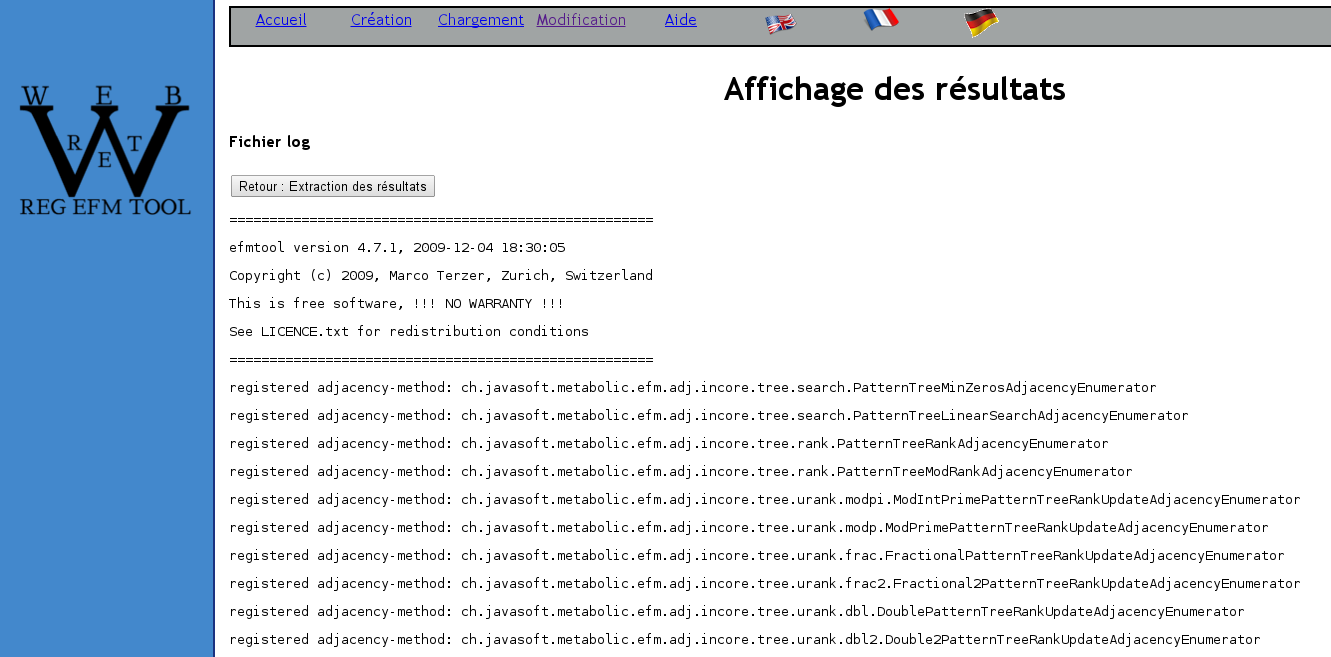
\includegraphics[width=0.90\textwidth]{../Images/Rapport/affichageResultats.png}  
		 \end{minipage}}
		\caption{Page de recherche sur le log}
  		\label{affichageResultats}
  	\end{center}	
\end{figure}

Nous avons tenté de faire en sorte que les résultats extraits soient affichés de façon claire et lisible pour l'utilisateur grâce au fichier \emph{display\_results.php}. Ce dernier récupère le mot-clé sélectionné dans le menu déroulant de la page précédente et le recherche dans l'ensemble du fichier. Si ce dernier comporte un 'R', seule la ligne comportant le mot clé est retournée. Dans le cas contraire, un des mot-clé suivant délimitera la catégorie sélectionnée. Cette recherche offre deux possibilités grâce à la fonction \texttt{display\_results()} du fichier \emph{display\_results.php}:
\begin{itemize}
\item dans le premier cas, si le mot-clé est suivi d'autres mots-clés contenant eux-même un 'R', le mot-clé délimitant sera le premier qui ne possédera pas de 'R',
\item dans le second cas, le mot-clé suivant dans la liste, servira de délimitant.
\end{itemize}

Nous avons également ajouté un bouton permettant de retourner sur la page d'extraction des résultats (Figure \ref{affichageExtraction}).

\begin{figure}[!ht]
	\begin{center}
		\fbox{
   		 \begin{minipage}[c]{0.3\textwidth}
  			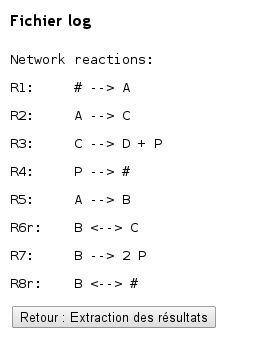
\includegraphics[width=0.8\textwidth]{../Images/Rapport/affichageExtraction.png}  
		 \end{minipage}}
		\caption{Exemple de recherche sur le log}
  		\label{affichageExtraction}
  	\end{center}	
\end{figure}

%%%%%%%%%%%%%%%%%%%%%%%%%%%%%%
\chapter{Difficultés et améliorations}
%%%%%%%%%%%%%%%%%%%%%%%%%%%%%%

Nous allons maintenant voir les difficultés que nous avons rencontré au cours de ce projet, ainsi que les améliorations possibles. \\

Suivant le navigateur utilisé, la récupération des fichiers par la fonction \texttt{move\_uploaded\_file()} ne fourni pas le m\^eme résultat, en particulier pour le dossier récupérant les fichiers. \\
De plus, il semblerait que les variables permettant de récupérer les fichiers \texttt{\$FILES} ne fonctionnent pas sur toutes les configurations. Jusqu'à présent, nous n'avons pas compris quel facteur influençait l'utilisation de ces variables et n'avons pas pu exécuter \textit{regEfmtool} depuis l'interface sur toutes les machines. \\
Les variables de sessions PHP étant propres à ce langage, nous avons parfois dû utiliser les cookies, en particulier lorsque certaines valeurs devaient \^etre sauvegardées depuis un script \emph{JavaScript}. Cela provoque l'utilisation de ces deux types de variables, ce qui n'est pas très uniforme. \\
L'affichage des résultats n'a été fait que superficiellement, d'où la présence de \textit{mode élémentaire 0} devant les noms de réactions, ou encore un simple affichage en tableau des résultats brut, indiquant la présence de réactions avec une valeur à 0 (c'est à dire non représentées dans les modes élémentaires). L'amélioration de cette partie ne devant pas être trop gourmande en temps mériterait d'\^etre modifiée. \\
Pour finir, l'utilisation de \textit{regEfmtool} depuis l'interface que nous avons créé dépend de la configuration du serveur Web installé sur la machine. Dans notre cas les tests étaient fait sous \emph{apache2} sur nos machines personnelles (la configuration du serveur sur les machines du \emph{CREMI} étant trop restrictives, il nous était impossible d'exécuter le logiciel).



